\documentclass[] {article}
\usepackage{amsmath}
\usepackage{graphics}
\usepackage{graphicx}
\usepackage[margin=2.5cm]{geometry}
\usepackage{color}
\usepackage{fancyhdr}
\usepackage{geometry}


\title{The Consistency Keys: A  Full Risk-Management System for Forex Trading}
\author{MR5OBOT \\ \textit{"It starts by hard work, but it's end with the smart work."}}
\begin{document}
\date{\today}
\maketitle
\pagestyle{fancy}
\tableofcontents 
\newpage


\begin{figure}[h]
    \centering
    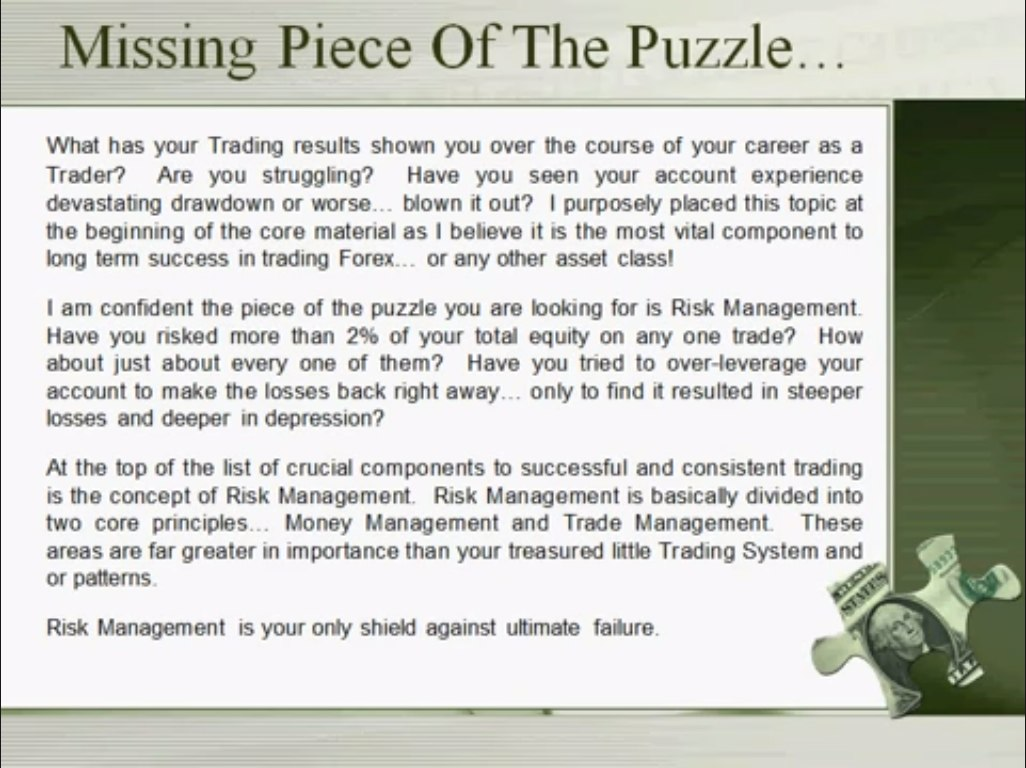
\includegraphics[width=1\textwidth]{./assets/the_missing_puzzel.jpg}
    \caption{The missing puzzel}
    \label{fig:puzzel}
\end{figure}

\vspace{0.5cm}

\noindent \textbf{\underline{Note:}}
\small{Always remember, if you can't follow the rules you will never be consistent even if you have a higher Win-Rate up to 90\%, bc with just one trade you can blow any account if you don't have the proper way of managin risks.
}

\vspace{1cm} % Adjust the vertical space as needed

\noindent \textbf{\underline{Disclaimer:}}
\small{The content presented in this paper is provided for informational and educational pur-
poses only and should not be considered as financial or investment advice. The author of this paper is
not a licensed financial professional, and the information contained herein should not be interpreted as
a recommendation, endorsement, or solicitation to engage in any financial or investment activity. The
views and opinions expressed in this paper are those of the author and do not represent the views of
any financial institution, regulatory body, or other organization. The author assumes no responsibility
for any financial losses, damages, or consequences resulting from the use of the information provided
in this paper.}

\newpage

\subsection{Risk Management}
\subsection{Money Management}
\subsection{Money Management Example}

\newpage
\section{Formulas}

\subsection{The combination of Risk-reward and Winrate} \vspace{0.8cm}

\[ \text{RR Formula}\ =\ \frac{\text{Win Rate}}{\text{1}\text{ - Win Rate}} \] \

\[ \text{Winrate Formula}\ =\ \frac{\text{Risk}}{\text{Risk} + \text{Reward}}\] \

\begin{itemize}
    \item Missing piece of puzzel
    \item Risk-Management explanation
\end{itemize}

 


\end{document}
